%! Author = janwi
%! Date = 11.01.2025

% Preamble
\documentclass[11pt]{article}
\usepackage[a4paper, total={6in, 8in},headsep=1cm]{geometry}
\usepackage{fancyhdr}
\usepackage[german]{datetime}
\usepackage{amsmath}
\usepackage{blindtext}
\usepackage{float}
\usepackage[bottom]{footmisc}
\usepackage{tikz}
\usepackage[tight,footnotesize]{subfigure}

\usepackage[utf8]{inputenc}
\usepackage{fourier}
\usepackage{array}
\usepackage{makecell}

\renewcommand\theadalign{bc}
\renewcommand\theadfont{\bfseries}
\renewcommand\theadgape{\Gape[4pt]}
\renewcommand\cellgape{\Gape[4pt]}



\usepackage[ngerman]{babel}
\usepackage{graphicx}
%\geometry{a4paper, margin=2.5cm}
\usepackage{subcaption}
\usepackage{hyperref}
\usepackage{enumitem}
\usepackage{hhline}
\hypersetup{
    colorlinks,
    linkcolor={blue!50!black},
    citecolor={blue!50!black},
    urlcolor={blue!80!black}
}



\oddsidemargin=-1cm
\voffset=-1.7cm
\textheight=26cm
\textwidth=18cm

\fancyhf{} % clear all fields
\newcommand{\footl}{}
\newcommand{\headl}{Sponsoring WRO Phoenix}

\fancypagestyle{plain}{%
    \fancyhf{}
    \fancyhead[L]{\rule[-2ex]{0pt}{2ex}\small \headl}
    \fancyhead[R]{\small \today}
    \fancyfoot[L]{\small \footl}
    \fancyfoot[C]{-- \thepage\ --}
    \fancyfoot[R]{\small }
    \renewcommand{\headrulewidth}{0.2pt}
    \renewcommand{\footrulewidth}{0.2pt}}
\pagestyle{plain}

\title {\vspace{-1cm} \huge \textbf {Unterstützen Sie das WRO Phoenix Team!}}

\author{}
\date{}

% Document
\begin{document}
    \vspace{-1cm}
    \maketitle
    \vspace{-1cm}


    % \section*{Einleitung}

    \noindent Wir, das WRO Phoenix Team, beschäftigen uns seit Jahren in der Freizeit mit Robotik und sind begeistert von den praktischen Anwedung und tüfteln auch sehr gerne.
    Wir nehmen 2025, zum vierten Mal, an der \href{https://wro.swiss/}{World Robotics Olympiad}\footnote{\href{https://wro.swiss}{https://wro.swiss}} (WRO) teil – einem internationalen Robotik-Wettbewerb, bei dem Jugendliche in kleinen Teams Roboter entwickeln und programmieren. In unserer Kategorie, der Robomission, muss ein autonomer Roboter innerhalb von zwei Minuten auf einem Spielfeld selbstständig verschiedene Aufgaben bewältigen, wie zum Beispiel das Erkennen, Verschieben oder Sortieren von Objekten auf dem Spielfeld.
    \vspace{0.2cm}
    \\
    In den vergangenen Jahren durfte der Roboter ausschliesslich mit einem Lego-Robotik-Set und anderen Lego-Komponenten gebaut werden. Dieses Jahr jedoch sind auch weitere Materialien und Technologien zugelassen. Dadurch eröffnen sich viele neue Möglichkeiten, unseren Roboter zu verbessern – wofür wir nun finanzielle Unterstützung von ungefähr 2000 CHF benötigen.
    \vspace{0.2cm}
    \\
    Damit wir die neuen Möglichkeiten ausschöpfen und der Konkurrenz standhalten können, würden wir uns sehr über Ihre Unterstützung als Sponsor freuen.

    \section*{Wer sind wir?}
    \begin{center}
        \begin{minipage}{\linewidth}
            \begin{figure}[H]
                \centering
                \begin{minipage}{0.31\linewidth}
                    \centering
                    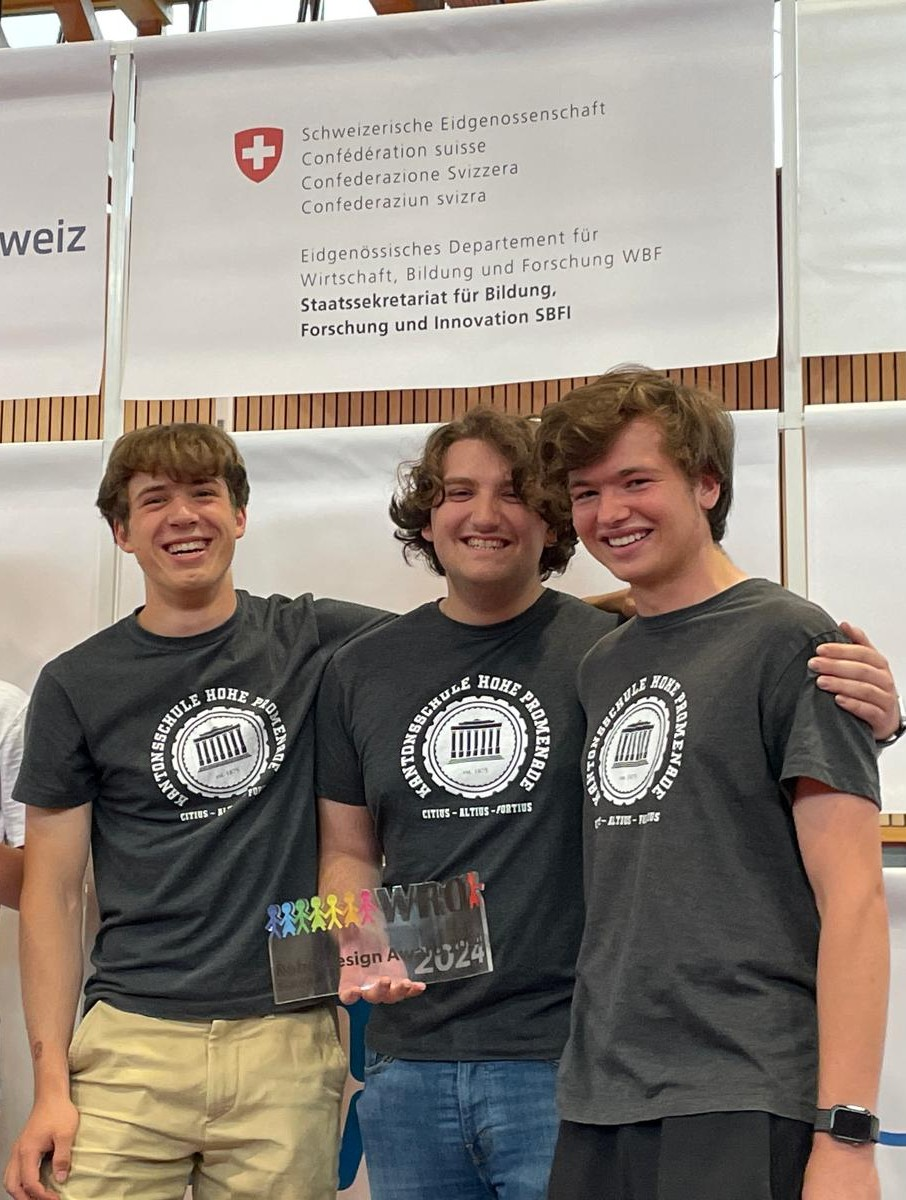
\includegraphics[width=.9\linewidth]{./team}
                    \caption*{\centering Phoenix Team mit Design Award}
                \end{minipage}%
                \begin{minipage}{.1\linewidth}
                \end{minipage}%
                \begin{minipage}{.59\linewidth}
                    \includegraphics[width=.835\linewidth]{robot_karim.png}
                    \caption*{\centering \hspace{-1cm} Karim am Bauen}
                \end{minipage}
            \end{figure}
        \end{minipage}
    \end{center}
    \begin{itemize}
        \item \textbf{Lucien Kissling (links):} Maturand an der Kantonsschule Hohe Promenade Zürich
        \item \textbf{Karim Freytag (Mitte):} Informatik-Student an der ETH Zürich, ehemalig Kantonsschule Hohe Promenade Zürich
        \item \textbf{Jan Wilhelm (rechts):} Maturand an der Kantonsschule Hohe Promenade Zürich
    \end{itemize}


    \section*{Unsere bisherigen Erfolge an der World Robotics Olympiad}
    \begin{itemize}
        \item \textbf{2024}: 5.
        Platz schweizweit, 1.
        Platz Design-Award, 11.
        Platz Open Championship in Brescia, Italien\footnote{\href{https://scoring.wro-association.org/en/regular2019/projector/169/4}{https://scoring.wro-association.org/en/regular2019/projector/169/4}}
        \item \textbf{2023}: 6.
        Platz schweizweit (trotz Abwesenheit zweier Teammitglieder aufgrund von Austauschsemester)
        \item \textbf{2022}: 4.
        Platz schweizweit
    \end{itemize}

    \noindent Unsere bisherigen Teilnahmen haben uns wertvolle Erfahrungen gebracht, und wir sind überzeugt, dieses Jahr noch besser abschneiden zu können.

    \section*{Warum wir Sponsoren brauchen}

    Bislang war der Wettbewerb auf Lego beschränkt, was die Kosten niedrig hielt.
    Mit den neuen Regeln, ab 2025, müssen wir jedoch verschiedene Materialien, Bauteile und Technologien einsetzen.
    Dies macht die Teilnahme nicht nur anspruchsvoller, sondern auch kostenintensiver.

    \section*{Wofür wird das Geld verwendet?}

    \subsection*{Geschätzte Kosten:}\\

    \begin{center}
        \begin{tabular}{|c|c|}
            \hline
            \textbf{Bereich} & \textbf{Kosten (CHF)} \\
            \hline
            Bauteile         & 700                   \\
            Ersatzbauteile   & 500                   \\
            Material         & 300                   \\
            Werkzeuge        & 300                   \\
            Weitere Kosten   & 200                   \\
            \hline
            Total            & 2000                  \\
            \hline
        \end{tabular}
    \end{center}

    \noindent Detailliertere Information zu den Kosten sind im Anhang zu finden.


    \section*{Unser Ziel}
    \begin{itemize}
        \item Top Platzierung an der Schweizer Meisterschaft mit Qualifikation f\"urs Weltfinale in Singapur oder für die Open Championship in Slowenien
        \item Platzierung im ersten Drittel am Weltfinale in Singapur oder an der Open Championship in Slowenien
    \end{itemize}

    \section*{Warum wir erfolgreich sein können}

    Wir starten dieses Jahr unter gleichen Bedingungen wie alle anderen Teams, da die Regeln neu sind.
    Unsere bisherigen Herausforderungen mit Lego-bedingten Ungenauigkeiten können wir dank moderner Materialien und Bauteile endlich überwinden.
    Unser Wissen und unsere Erfahrung im Bereich Robotik und Informatik haben wir auch dank unserer Maturarbeiten in diesen Bereichen in letzter Zeit weiter ausgebaut.

    \begin{figure}[h]
        \centering
        \includegraphics[width=0.7\linewidth]{robot.png}
        \caption*{WRO Phoenix Roboter in Aktion beim Open Championship Turnier in Brescia}
        \label{fig:robot}
    \end{figure}

    \section*{Sponsoring-Pakete}
    Falls Sie uns unterstützen möchten gibt es verschieden Möglichkeiten:

    \textbf{1. Silber-Sponsor (ab 200 CHF)}
    \begin{itemize}
        \item Kleines Logo auf unserem Roboter
    \end{itemize}

    \noindent\textbf{2. Gold-Sponsor (ab 500 CHF)}
    \begin{itemize}
        \item Grosses Logo auf unserem Roboter
        \item Kleines Logo auf unseren Team-T-Shirts
    \end{itemize}

    \noindent\textbf{3. Platin-Sponsor (ab 1000 CHF)}
    \begin{itemize}
        \item Grosses Logo auf unserem Roboter
        \item Grosses Logo auf unseren Team-T-Shirts (Hauptsponsor)
    \end{itemize}

    \noindent Gerne tauschen wir uns mit Ihnen über ihre Vorstellungen aus.

    % \noindent\textbf{4. Exklusiv-Sponsor (2000 CHF bis zur Schweizer Meisterschaft)}
    % \begin{itemize}
    %     \item Exklusives Sponsoring (nur Ihr Logo und unser WRO Phoenix Logo)
    %     \item Bei Qualifikation für einen internationalen Wettbewerb: Abdeckung weiterer Kosten (für die Reise und Weiterentwicklung vom Projekt) je nach Destination bis zu zusätzlich 5000 CHF
    %     \item Grosses Logo auf Roboter und T-Shirts
    %     \item Logo auf allen Materialien und Präsentationen
    % \end{itemize}

    \section*{Kontakt}

    Für Fragen und weitere Informationen stehen wir Ihnen gerne zur Verfügung:

    \noindent \textbf{E-Mail:} team.wro.phoenix@gmail.com\\
    \textbf{Telefon:} +41 78 699 20 50\\
    \vspace{0.2cm}\\
    \noindent Es würde uns sehr freuen, auf Sie als Sponsor zählen zu können.
    \newpage

    \section*{Anhang}
    Bericht unserer Schule vom Jahr 2022:
    \href{https://kshp.ch/buchstabenseiten/k-wie-konzert-2-1}{Kantonsschule Hohe Promenade Zürich Bericht}
    \\ \\
    Unsere Maturitätsarbeiten
    \begin{itemize}[label={}]
        \item Jan Wilhelm: \href{https://kshp.phoenix-network.dev/MA_Jan_Wilhelm.pdf}{Designing, assembling and programming
        a foosball goalkeeper robot}\footnote{\href{https://kshp.phoenix-network.dev/MA_Jan_Wilhelm.pdf}{https://kshp.phoenix-network.dev/MA\_Jan\_Wilhelm.pdf}}
        \item Karim Freytag: \href{https://kshp.phoenix-network.dev/MA_Karim_Freytag.pdf}{Model of a Self-Balancing Bike
        }\footnote{\href{https://kshp.phoenix-network.dev/MA_Karim_Freytag.pdf}{https://kshp.phoenix-network.dev/MA\_Karim\_Freytag.pdf}}
        \item Lucien Kissling: \href{https://kshp.phoenix-network.dev/MA_Lucien_Kissling.pdf}{Evolutionary Neural Networks:
        Designing a NEAT-Inspired Algorithm
        for Strategic Game Learning
        }\footnote{\href{https://kshp.phoenix-network.dev/MA_Lucien_Kissling.pdf}{https://kshp.phoenix-network.dev/MA\_Lucien\_Kissling.pdf}}
    \end{itemize}


    \newpage
    \subsection*{Genauere Kosten}
    \textbf{Details der Bauteile:}
    \vspace{0.2cm}\\
    \begin{tabular}{|c|c|c|c|c|}
        \hline
        \textbf{Anzahl} & \textbf{Bauteil} & \thead{\textbf{Kosten pro Teil (CHF)}} & \textbf{Kosten total (CHF)} & Total \\
        \hline
        \multicolumn{5}{|r|}{\textbf{}} \\
%        \hline
        \multicolumn{5}{|c|}{\textbf{\underline{Bauteile}}} \\
        \hline
        5 & \href{https://www.dfrobot.com/product-1462.html}{DC Motor}                                                          & 30  & 150  & \\
%        \hline
        2 & \href{https://www.dfrobot.com/product-2142.html}{BNO055 (IMU)}                                           & 18 & 36  & \\
%        \hline
        6 & \href{https://www.pololu.com/product/1425}{Rad}                                              & 6  & 36  & \\
%        \hline
        2 & \href{https://www.basicmicro.com/Roboclaw-2x7A-Motor-Controller_p_55.html}{Roboclaw}                                              & 80  & 160  & \\
%        \hline
        5 & \href{https://www.dfrobot.com/product-540.html}{Farbsensor}                                              & 8  & 40  & \\
%        \hline
        4 & \href{https://www.bastelgarage.ch/tower-pro-micro-servo-9g-sg90-1-150}{Servomotor} & 5 & 20 &\\
%        \hline
        2 & \href{https://www.digitec.ch/en/s1/product/isdt-dual-charger-p10-rc-chargers-13944492}{Ladegerät} & 52 & 105& \\
%        \hline
        2 & \href{https://www.joom.com/de/products/64cf5e243899ad01e54e2332}{Batterie-Managementsystem} & 4 & 8 &\\
%        \hline
        2 & \href{https://www.amazon.de/HRB-4000mAh-Battery-Batteries-Compatible/dp/B0BYRHDHHY}{Batterie}                                         & 28 & 56  & \\
%        \hline
        1 & \href{https://www.amazon.com.be/-/en/Pairs-Female-Connector-Silicone-12AWG/dp/B07QH249CR}{Batteriekabel}                                                                                                          & 9    & 9     & \\
%        \hline
        2 & \href{https://www.pi-shop.ch/raspberry-pi-camera-3-wide}{Pi Cam} & 40 & 80 & \\
%        \hline
%        & & & & \\
        \hline
        \multicolumn{4}{|r|}{\textbf{Gesamtkosten Bauteile}} & \textit{700} \\
        \hline
        \multicolumn{5}{|r|}{\textbf{}}  \\
%        \hline
        \multicolumn{5}{|c|}{\textbf{\underline{Ersatzbauteile}}}  \\
        \hline
        & Ersatzmotoren                                                                                                 &    & 100 & \\
        & Zusätzliche Motoren für Aufgaben                                                                         &    & 200 & \\
        & Sensoren & & 100 & \\
        & Restkosten (Kabel, Stecker etc.) & & 100 & \\
        \hline
        \multicolumn{4}{|r|}{\textbf{Gesamtkosten Ersatzbauteile}} & \textit{500} \\
        \hline
        \multicolumn{5}{|r|}{\textbf{}}  \\
%        \hline
        \multicolumn{5}{|c|}{\textbf{\underline{Materialkosten}}}  \\
        \hline
        & D-Druck-Material (PLA, Nylon, Resin) & & 250 & \\
        & Aluminium oder andere CNC-Materialien & & 50 & \\
        \hline
        \multicolumn{4}{|r|}{\textbf{Gesamtkosten Material}} & \textit{300} \\
        \hline
        \multicolumn{5}{|r|}{\textbf{}} \\
%        \hline
        \multicolumn{5}{|c|}{\textbf{\underline{Werkzeuge}}} \\
        \hline
        \multicolumn{4}{|r|}{\textbf{Gesamtkosten Werkzeuge (Löhtkolben, Powersupply)}} & \textit{300} \\
        \hline
        \multicolumn{5}{|r|}{\textbf{}}  \\
%        \hline
        \multicolumn{5}{|c|}{\textbf{\underline{Adminkosten}}}  \\
        \hline
        & Anmeldung & & 100 & \\
        & Team T-Shirt & & 100 & \\
        \hline
        \multicolumn{4}{|r|}{\textbf{Gesamtkosten Adminkosten}} & \textit{200} \\
        \hline
        \multicolumn{5}{|r|}{\textbf{}} \\
        \hline
        \multicolumn{4}{|r|}{\textbf{Gesamtkosten Total}} & \textit{\underline{2000}} \\
        \hline
    \end{tabular}

\end{document}
